\documentclass[12pt]{article}
\usepackage[hidelinks]{hyperref}
\usepackage[italian]{babel}
\usepackage{graphicx}
\usepackage{outlines}
\begin{document}
\tableofcontents
\newpage

\section{Introduzione}
\subsection{Motivazione} 
Un linguaggio è uno strumento per descrivere come risolvere i problemi in maniera rigorosa, in modo tale che sia eseguibile da un calcolatore
Perché è utile studiare come creare un linguaggio di programmazione? 
\begin{itemize}
  \item non rimanere degli utilizzatori passivi
  \item capire il funzionamento dietro le quinte di un linguaggio
  \item domain-specific language (DSL): è un linguaggio pensato per uno specifico problema
  \item model drivern software development: modo complesso per dire UML e simili
  \item model checking
\end{itemize}


\subsection{Definizioni base} 
Un linguaggio è composto da:
\begin{itemize}
  \item lessico e sintassi
  \item compilatore: parser + generatore di codice oggetto
\end{itemize}
La generazione automatica di codice può essere dichiarativa lessico
(espressioni regolari o automa a stati finite) o sintassi(grammatiche o automa a pile).
Un automa a stati finiti consuma informazioni una alla volta, ne salva una quantità finita. Alcuni esempi di applicazione di automa a stati finiti: software di progettazione di circuiti, analizzatore lessicale, ricerca di parole sul web e protocolli di comunicazione.
\begin{figure}[h]
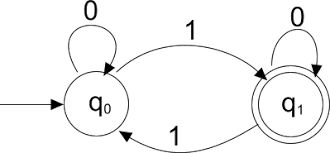
\includegraphics[scale = 0.3]{media/semplice_automa.png}
\centering
\caption{Semplice automa}
\end{figure}

\subsection{Contenuti del corso}
\begin{outline}
  \1 Linguaggi formali e Automi:
    \2 Automi a stati finiti, espressioni regolari, grammatiche libere, automi a pila, Macchine di Turing, calcolabilità
  \1 Compilatori:
    \2 Analisi lessicale, analisi sintattica, analisi semantica, generazione di codice
  \1 Logica di base:
    \2 Logica delle proposizioni e dei predicati
  \1 Modelli computazionali:
    \2 Specifica di sistemi tramite sistemi di transizione, logiche temporali per la specifica e verifica di proprietà dei sistemi (model checking), sistemi concorrenti (algebre di processi e reti di Petri)
\end{outline}

\subsection{Informazioni utili}
Parte integrante del corso:
\begin{outline}
  \1 Supporto alla parte teorica usando tool specifici.
  \2 JFLAP 7.1: http://www.jflap.org (automi/grammatiche)
  \2 Tina 3.7.5: http://projects.laas.fr/tina
  (model checking di sistemi di transizione e reti di Petri)
  \2 LTSA 3.0: http://www.doc.ic.ac.uk/ltsa
  (sistemi di transizione definiti tramite algebre di processi)
  \1 Nel resto del corso utilizzeremo un ambiente di sviluppo per
  generare parser/compilatori
  \2 IntelliJ esteso con plug-in ANTLRv4, ultima versione 1.20
  (generatore ANTLR: http://www.antlr.org/)
\end{outline}

\newpage
Libri di testo suggeriti:
\begin{outline}
 \1 J. E. Hopcroft, R. Motwani e J. D. Ullman:
Automi, linguaggi e calcolabilita’,
Addison-Wesley, Terza Edizione, 2009. Cap. 1–9
\1 A. V. Aho, M. S. Lam, R. Sethi e J. D. Ullman:
Compilatori: principi tecniche e strumenti,
Addison Wesley, Seconda Edizione, 2009. Cap. 1–5
\1 M. Huth e M. Ryan:
Logic in Computer Science: Modelling and Reasoning about
Systems,
Cambridge University Press, Second Edition, 2004. Cap. 1–3 
\end{outline}

\newpage
\section{Linguaggi regolari}

\end{document}

